% 2011 年山东卷文科第 22 题：椭圆 C、直线 l、射线 OE 与直线 x = -3。
% 来源 PDF：普通高考/2011/2011山东文.pdf，SHA-256 bf61cf7bb39a3ccfc57735cd2a7ab34387cbfa6bc86a5e7f8246e13292b0e023。
% 原页：第 2 页（A3 三栏）第 3 栏中部，书页码 692。
% 重绘依据：原页矢量层实测定标——椭圆外框 x∈[-49.08,49.08]pt、y∈[-28.34,28.34]pt，
%   半长轴∶半短轴 = 49.08∶28.34 ≈ √3∶1，与题设 x²/3+y²=1 完全一致，故取 28.34pt = 1 单位；
%   竖直直线 x=-3 在原页实测位于 -85.01pt = -3 单位，印证该定标。
%   原页要素（单位坐标）：x 轴自 -3.50 到 2.17，y 轴自 -2.00 到 2.27；
%   直线 x=-3 自 y=2.20 到 -1.80；射线 OE 与直线 l 均画到图形之外，照原页截断。
%   本图按几何自洽重排：取 l:y=0.8x+0.5（k>0、不过原点），与椭圆 x²/3+y²=1 交于
%   A(0.5583,0.9466)、B(-1.3802,-0.6042)，中点 E(-0.4110,0.1712)；
%   射线 OE 的斜率为 -0.4167，交椭圆于 G(-1.4045,0.5852)、交 x=-3 于 D(-3,1.2500)。
%   沿射线自 O 向外的次序为 E、G、D，与原页一致；l 的两端各伸出椭圆之外。
%   标注位置照原页相对格局（D 在竖线右侧上方、G 在 OE 与椭圆交点外上侧、E 在交点下方、
%   A 在右上交点外侧、B 在左下交点外侧、O 在原点右下、-3 在 x 轴下方竖线左侧、l 在右上方）。
%   全图无网格、无辅助虚线。
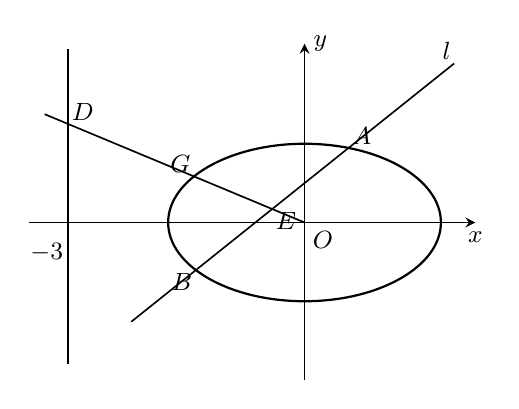
\begin{tikzpicture}[x=1cm, y=1cm, >=stealth, semithick, font=\small]

  % ===== 坐标轴 =====
  \draw[->] (-3.50,0) -- (2.17,0) node[below, inner sep=3pt] {$x$};
  \draw[->] (0,-2.00) -- (0,2.27) node[right, inner sep=3pt] {$y$};

  % ===== 椭圆 =====
  \draw[thick] (0,0) ellipse ({sqrt(3)} and 1);

  % ===== 直线 x = -3 =====
  \draw (-3,2.20) -- (-3,-1.80);

  % ===== 射线 OE（过 O、E、G、D 的直线，画到 D 之外）=====
  \draw (0,0) -- (-3.30,1.3751);
  % ===== 直线 l（过 A、B，两端伸出椭圆）=====
  \draw (-2.20,-1.2600) -- (1.90,2.0200);

  % ===== 标注 =====
  \node[above right, inner sep=1pt] at (-3,1.2500) {$D$};
  \node[above left, inner sep=1pt] at (1.90,2.0200) {$l$};
  \node[above left, inner sep=1pt] at (-1.4045,0.5852) {$G$};
  \node[above right, inner sep=1pt] at (0.5583,0.9466) {$A$};
  \node[below right, inner sep=1pt] at (-0.4110,0.1712) {$E$};
  \node[below right, inner sep=1pt] at (0.06,-0.07) {$O$};
  \node[below left, inner sep=1pt] at (-1.3802,-0.6042) {$B$};
  \node[below left, inner sep=1pt] at (-3.02,-0.22) {$-3$};

\end{tikzpicture}
